% ---------------------------------------------------------------------------------%
%  Description: Project Report of the FAI-TANGO Android App	%
%                                                                              				%
%  Author(s): chris                                                            			%
%  Date: 31 March 2012 20.40                                                   	%
% --------------------------------------------------------------------------------	%

\documentclass[12pt, twoside]{article}

% -------------------------------------------------------------------------------- %
% Including Packages                        						%
% --------------------------------------------------------------------------------	%
\usepackage{fullpage} % To use 1 inch margins
%\usepackage{latex8}
%\usepackage{ieeetran}
\usepackage{color}
\usepackage{times}
\usepackage{url}
\usepackage{amsfonts}
\usepackage{amsmath}
\usepackage{graphicx}
%\usepackage{../../Styles/algorithm}
%\usepackage{../../Styles/algorithmic}
\usepackage{algorithm}
\usepackage{algorithmic}
\usepackage{theorem}
\usepackage{multirow}
\usepackage{epsf}
\usepackage{psfrag}
\usepackage{latexsym}
\usepackage{lscape}

% ----------------------------------------- %
% New commands and environments             %
% ----------------------------------------- %
\newcommand{\todo}[1]{{\color{red}{TODO: \textbf{\footnotesize{#1}}}}}

\newcommand{\app}{FAI-TANGO }

\renewcommand{\labelenumi}{\arabic{enumi}}
\renewcommand{\labelenumii}{\arabic{enumi}.\arabic{enumii}}
\renewcommand{\labelenumiii}{\arabic{enumi}.\arabic{enumii}.\arabic{enumiii}}

% ----------------------------------------- %
% Body (Title, author, abstract, sections)  %
% ----------------------------------------- %
%\graphicspath{{../figures/}}
%\DeclareGraphicsExtensions{.jpg}
%\DeclareGraphicsExtensions{.eps}
%\pagestyle{empty}
\title{\app Android App}
\author{Juri Lelli, Stefano Fontanelli, Christian Nastasi} 

\begin{document}
\maketitle
%\thispagestyle{empty}
% ----------------------------------------- %
% Abstract of the document                  %
% ----------------------------------------- %
%\begin{abstract} There is no abstract.  \end{abstract}

% ----------------------------------------- %
% Add document sections                     %
% ----------------------------------------- %
Topics:
\begin{itemize} 
    \item Introduction: about the app
    \item Requirements of the app
    \item General Architecture:
    \begin{itemize} 
        \item Local DB to store event information
        \item Module for information retrieval
        \item Module for information presentation
        \item Integration with Android: maps, calendar, facebook
    \end{itemize} 
    \item SW architecture: (basically the java packages) 
    \begin{itemize} 
        \item DB module
        \item GUI module
        \item Synch module 
        \item Preferences 
    \end{itemize} 
    \item DB module: DB helper, Content provider
    \item GUI module: main Activity, event detail activity
    \item Synch module: retrieval (EventFetcher and EventParser), ReaderService!
    \item Preferences
\end{itemize} 
\normalsize


\section{Application description}

The \app application allows to retrieve and present information about
tango events registered at the \emph{FAItango} association 
(``Federazione delle Associazioni Italiane di Tango Argentino'').
Such information are available through the FAItango official web site,
but cannot be easily accessible on mobile handsets because of the lack of
a proper mobile version of the web site. 
Moreover, visualization through the web interface normally requires continuous
access to the internet.

The proposed application can be used to query the remote web site, store
events informations on the device and then display such informations in
a brief or detailed way. Additional features are event site visualization
through the Google Maps service, social sharing of an event details,
use of the Android integrated calendar to automatically add remainders.

\subsection*{Requirements}
\begin{enumerate}
	\item The tango event information is classified 
         		 in \emph{brief} and \emph{detailed}.
	\item Event whose starting date is previous than current date 
          	(handset time) are considered as \emph{past}.
    	\item	The application shall retrieve the event information from the 
          	FAItango database.
    		\begin{enumerate}
        			\item	\emph{Brief} and \emph{detailed} information are accessible through 
              			HTTP requests.
        			\item \emph{Brief} and \emph{detailed} information are encoded in JSON standard.
        			\item Information inside \emph{detailed} maybe encoded in plain HTML.
        			\item \emph{Brief} and \emph{detailed} information might be accessed and encoded using
              			different mechanisms.
    		\end{enumerate}
	\item The application shall present the event information on the handset.
    	\begin{enumerate}
        		\item The \emph{brief} information shall be summarized in a sorted list.
        			\begin{enumerate}
            			\item The list is sorted by event date, closest to current date first
            			\item Past events shall be excluded.
        			\end{enumerate}
        		\item The \emph{detailed} information shall be presented upon selection of
              		the event from the brief list.
    	\end{enumerate}
    	\item The application shall allow off-line visualization of the event information.
    		\begin{enumerate}
        			\item The application shall store \emph{brief} and \emph{detailed} information on the handset.
	        		\item Past events information should be removed.
    		\end{enumerate}
    	\item Information retrieval shall take place according to two possible 
          	paradigms: \emph{synchronization} and \emph{search}.
    	\item Synchronization
    		\begin{enumerate}
        			\item Synchronization shall accept search parameters to limit event information to be retrieved.
        				\begin{enumerate}
            				\item Information can be retrieved by country,
					\item	Information can be retrieved by country and province,
					\item	Information can be retrieved by country, province and municipality,
					\item	Information can be retrieved by event type (concert, festival, marathon, milonga, party, show, stage, vacation),
					\item	Information can be retrieved by time period (1 day, 7 days, 15 days, 1 month, 6 months, 12 month).
        				\end{enumerate}
        			\item Synchronization shall be performed in one of the following mode:
              			periodically, on-startup, manually.
				\begin{enumerate}
					\item Periodic synchronization shall occur according 
						predefined time interval (15 minutes, 30 minutes, 1 hour, 12 hours, 24 hours).
					\item Periodic synchronization shall occur even if the application is not executing.
            				\item On-startup synchronization shall occur when the application is started.
					\item Manual synchronization shall occur on explicit request of the user.
				\end{enumerate}
		\end{enumerate}
	\item Search
    		\begin{enumerate}
        			\item It shall be offline.
			\item It shall limit event information to be showed:
			\begin{enumerate}
				\item by country,
				\item	by country and province,
				\item	by country, province and municipality,
				\item by event type,
				\item by time period.
			\end{enumerate}
			\item It shall update synchronization parameters preference.
			\item	It shall ask the user to start synchronization when no result found.
    		\end{enumerate}
    	\item The application shall be integrated with: calendar, maps, social networks.
    	\item The application shall provide off-line content to other possible application.
\end{enumerate}

\section{Architecture}

The architecture proposed to comply with the application requirements
is depicted in Figure~\ref{fig:apparc}. 

The main parts of the application are:
\begin{enumerate}
	\item	the event list activity,
	\item	the event details activity,
	\item	the preference activity,
	\item	the set of data providers,
	\item	the updater service.
\end{enumerate}

\begin{figure}[h]
\begin{center}
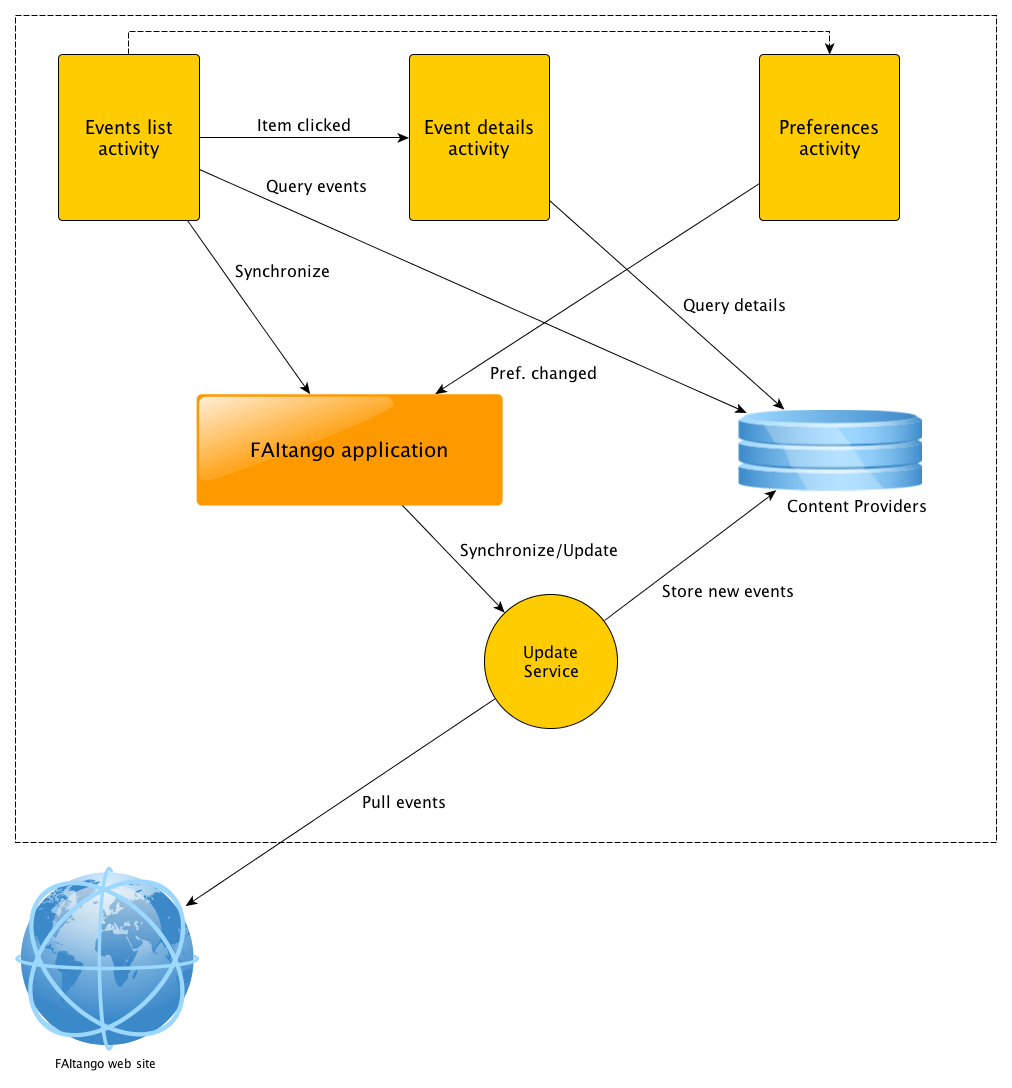
\includegraphics[scale=0.39]{fig/app_structure.png}
\end{center}
\caption{The application architecture}
\label{fig:apparc}
\end{figure}


\subsection{The event list activity}

The event list activity shows \emph{brief} information about events, grouped and ordered by data.
An example can be viewed in Figure~\ref{fig:eventlist} and Figure~\ref{fig:eventlistmenu}: the list is a collapsed set of dates when it is displayed. Each item in the list can be clicked to display a list of \emph{brief} information about events that will take place that day. Each item inside that list is clickable too and the click event display the \emph{event detail activity}.

\begin{figure}[h]
\begin{center}
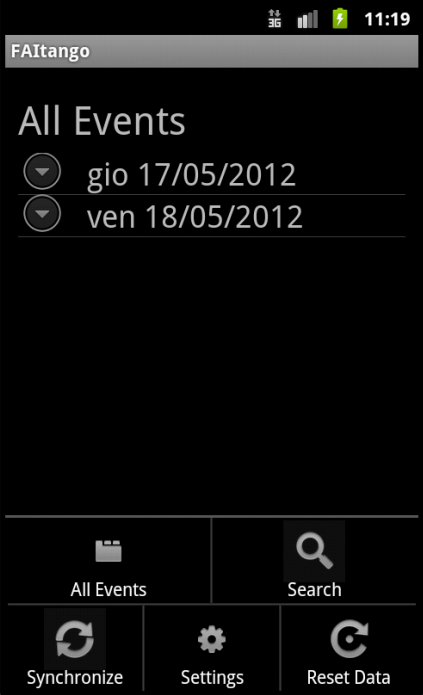
\includegraphics[scale=0.60]{fig/event-list-activity.png}
\end{center}
\caption{The event list activity's menu}
\label{fig:eventlistmenu}
\end{figure}

\begin{figure}[h]
\begin{center}
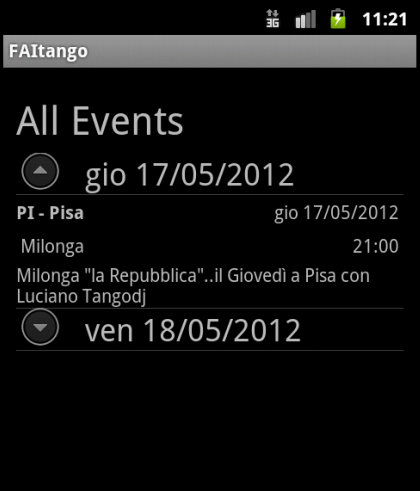
\includegraphics[scale=0.60]{fig/allevents-brief.png}
\end{center}
\caption{The event list activity}
\label{fig:eventlist}
\end{figure}

Users can access application functionalities through the menu of the event list activity, which is shown in Figure~\ref{fig:eventlistmenu}: the ``All Events'' option update the list to display all events stored in the local database, ``Search'' option display the \emph{search activity}, ``Synchronize'' run retrieving of \emph{brief} and \emph{detailed} infomation about events from remote server, ``Settings'' show the \emph{preference activity}, ``Reset Data'' drops events data from the local database.

\subsection{The event detail activity}

The event detail activity shows \emph{detailed} information about a specific event, as is shown in Figure~\ref{fig:eventdetailup} and Figure~\ref{fig:eventdetaildown}: it includes a long description with the location of the event and contact information. The activity includes a map which shows where event take place. The user can set a remainder in the agenda or share the event on social networks using buttons below the map.

TODO: parlare di come è fatto il reminder e lo share!

\begin{figure}[h]
\begin{center}
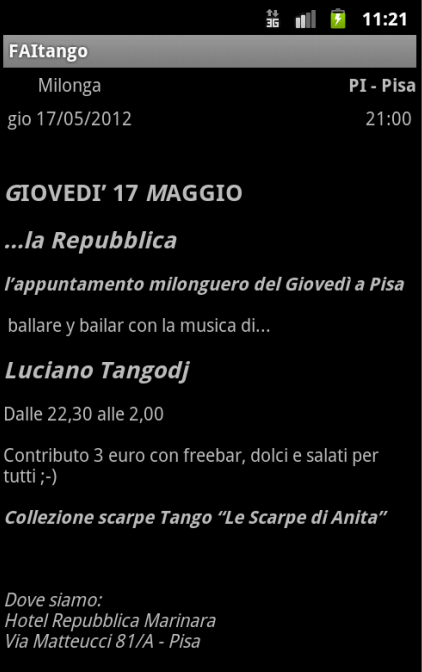
\includegraphics[scale=0.60]{fig/event-detail-up.png}
\end{center}
\caption{The event detail activity}
\label{fig:eventdetailup}
\end{figure}

\begin{figure}[h]
\begin{center}
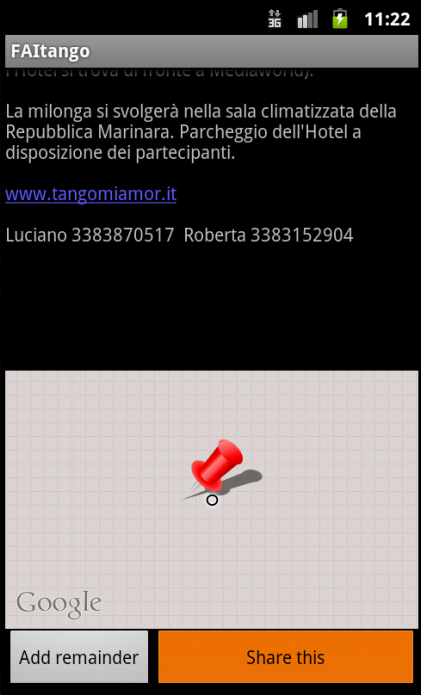
\includegraphics[scale=0.60]{fig/event-detail-down.png}
\end{center}
\caption{The event detail activity: google map and other buttons}
\label{fig:eventdetaildown}
\end{figure}

\subsection{The search activity}
TODO

\subsection{The preferences activity}
TODO

\subsection{The data providers}
TODO

\subsection{The updater service}

TODO

\end{document}
